\subsubsection{Data Requirements}
\label{sec:data_req}
One of the study's key objectives was data collection. As noted, the corpus was constructed to meet requirements
for universality and to support future research in related fields.

\textbf{Data Requirements.} Texts were chosen as the primary source of qualitative data. In the financial domain,
the most content-rich and impactful on asset prices are:

\begin{itemize}
    \item news articles;
    \item social-media posts;
    \item official reports (annual, quarterly, strategic);
    \item press releases;
    \item analytical reviews and articles;
    \item transcripts of interviews, conferences, and public-company webcasts.
\end{itemize}

Previous studies have validated the effectiveness of these text types. FinBERT \parencite{Yang2020FinBERT,Huang2023FinBERT},
for example, was trained on official reports and analytical articles, and its later versions incorporated press releases
\parencite{Liu2020FinBERT}. Other models have been successfully pre-trained on fragmented news articles and fine-tuned
for sentiment analysis on news headlines and social-media publications \parencite{Araci2019FinBERT}. Nevertheless,
our research deliberately processes full texts without fragmentation: official reports frequently exceed the 8,192
token limit of ModernBERT, complicating their integration, while very short formats (social-media posts) fail
to exploit the advantages of a long-context model.

Furthermore, no single source aggregates all of the above text types. Given limited resources, the following most
significant categories were selected for initial focus:

\begin{itemize}
    \item news articles;
    \item press releases;
    \item analytical reviews and articles;
    \item transcripts of financial events.
\end{itemize}

Expansion of the corpus to include additional content categories is planned for future work.

To ensure the corpus's versatility and facilitate subsequent use, the following metadata were collected for each text:

\begin{itemize}
    \item Headline (e.g., “Covestro board enters formal talks on \$12 billion ADNOC approach”);
    \item Source (copyright holder), e.g., Reuters, Simply Wall St., PR Newswire, @ilyasut, Max Gottich;
    \item Publication platform, e.g., Twitter, Yahoo! Finance, Reddit, Seeking Alpha;
    \item UTC timestamp with second-level precision (e.g., 2024-09-01T01:48:13);
    \item Author-assigned topical tags (e.g., [“M\&A”, “Cryptocurrency”, “Tech”])'
    \item List of tickers mentioned by the author (e.g., [“9626.HK”, “BILI”]).
\end{itemize}

Finally, the optimal period for data collection was established. The lower and upper bounds of the dates were selected
based on the assumption that this corpus will be used to train the value prediction model in the future, which requires
that the initial knowledge of ModernBERT be synchronized with those on which it will be fine-tuned later. Due to the fact
that the ModernBERT publication does not disclose the data on which the model was trained \parencite{Warner2024ModernBERT},
it is impossible to accurately judge for which period the data was taken. Therefore, in our study, focusing
on the date of ModernBERT publication \parencite{Warner2024ModernBERT} and the classical ratio of training,
validation and test samples as 75/15/10, we took the date range from September 17, 2023 to March 18, 2025, i.e. 548 days,
of which 374 are working days according to the US calendar.

\textbf{Source Requirements.} Data sources must be open, free, English-language, and authoritative, since wide
dissemination and timely publication directly affect market reactions. Considered sources included:

\begin{itemize}
    \item News outlets: Bloomberg\footnote{URL: \url{https://www.bloomberg.com/}},
    The New York Times\footnote{URL: \url{https://www.nytimes.com/}},
    Reuters\footnote{URL: \url{https://www.reuters.com/}}, etc;
    \item Analytical platforms: Seeking Alpha\footnote{URL: \url{https://seekingalpha.com/}},
    TradingView\footnote{URL: \url{https://tradingview.com/}};
    \item Official sites: Corporate and government portals.
\end{itemize}

An analysis of over 50 corporate and more than 100 government resources showed that, thanks to RSS feeds, press
releases are centrally aggregated via PR Newswire\footnote{URL: \url{https://www.cision.com/}} and
GlobeNewswire\footnote{URL: \url{https://www.globenewswire.com/}}. Other automated aggregators
(e.g., Business Wire\footnote{URL: \url{https://www.businesswire.com/}}) exist, but PR Newswire and GlobeNewswire
empirically dominate; however, they offer press releases only, without genre diversity.

Among news outlets, Reuters proved optimal in responsiveness and market coverage. Niche but high-quality sources
(e.g., The Information\footnote{URL: \url{https://www.theinformation.com/}}, Epoch AI\footnote{URL: \url{https://epoch.ai/}})
were also examined; they provide overly specialized content, whereas traditional outlets
such as Bloomberg, The Wall Street Journal\footnote{URL: \url{https://www.wsj.com/}},
and The Economist\footnote{URL: \url{https://www.economist.com/}} cover a broader market spectrum, albeit with
technical constraints.

Of the analytical platforms, Seeking Alpha was excluded due to its large volume of paywalled content, and TradingView
was unsuitable because it does not grant access to historical publications.

Thus, PR Newswire and Reuters became the corpus's primary sources. To mitigate the risk of systematic bias and ensure
broader coverage, it was nevertheless decided to enrich the corpus with additional publishers. Due to their fragmentation,
lack of APIs, and often incomplete metadata (including sub-second timestamps), aggregation and synchronization proved
unfeasible. Consequently, the aggregators Google Finance\footnote{URL: \url{https://www.google.com/finance/}},
Yahoo! Finance\footnote{URL: \url{https://finance.yahoo.com/}},
and FinURLs\footnote{URL: \url{https://finurls.com/}} were also considered.

Ultimately, Yahoo! Finance was selected thanks to its unified site structure and comprehensive aggregation of diverse
sources, whereas FinURLs redirects to individual source sites, each with its own layout. Google Finance, though similar
to Yahoo! Finance, does not support the collection of historical data.

\subsubsection{Data Collecting}
\label{sec:data_collecting}

Prior to data collection, a survey and analysis of existing open-source tools for harvesting data from Yahoo! Finance were conducted.
The analysis identified five candidate libraries. Two --- yahooquery and yahoo-stock-api --- do not support article extraction;
two others --- yahoo\_fin and fin-news --- are abandoned and no longer function correctly; and yfinance affords access only
to the latest twenty news items in real time. Consequently, a custom Python parser was developed. Its architecture comprises
two principal stages:

\begin{enumerate}
    \item Link Collection. A recursive traversal of the official sitemap is used to gather article URLs for a specified
    period. Each “daily page” lists 50 news links and a pointer to the next page; critically, page $n$ can only be accessed
    via page $n - 1$, creating a bottleneck akin to traversing a linked list under high network latency.
    \item Content Extraction. The gathered URLs are then parsed to extract each article's text. It should be noted that,
    as with training the original BERT model, tables and images are not processed \parencite{devlin2019BERT}.
\end{enumerate}

During development, several constraints were encountered and subsequently addressed in the parser's design:

\begin{itemize}
    \item IP-blocking and Cookies. Yahoo! Finance limits to 14 concurrent requests per IP at minimum 4-second intervals;
    violations yield HTTP 404, 429, or 200 responses with empty bodies. Even when these constraints are met, blocks may
    still occur. To mitigate this, a pool of 50 proxy servers was employed, and failed requests were automatically retried
    in subsequent iterations.
    \item Regional Restrictions. Identical URLs may be inaccessible or behave inconsistently when requested from different
    countries.
    \item Technical Errors. Redirects to external sources, broken links, and paywalled URLs were encountered and excluded
    during corpus assembly.
\end{itemize}

To accelerate processing of large datasets, the C-based library selectolax was used, offering roughly 30× the speed
of BeautifulSoup and 5× that of lxml.

As a result, the link-collection stage yielded 1,362,103 URLs, of which 1,360,761 belonged to the Yahoo! Finance domain.
Thanks to the parser's modular architecture, extensive proxy usage, and multiple iterations, 1,304,717 articles were
successfully parsed. The final corpus occupies 6.5 GB in CSV format and 2.2 GB in the more compact Parquet format.

The final class implementing the parser program can be found in the official repository of the project, called
YahooFinanceParser\footnote{URL: \url{https://github.com/denisalpino/FinABYSS}}.

\subsubsection{Data Analysis}
\label{sec:data_analysis}
Before commencing the pre-processing stage, it was decided to conduct a comprehensive analysis of the collected corpus of news articles.
This preliminary analysis not only revealed the characteristic features of the data but also established the foundation for subsequent
automation of text cleaning and structuring. Moreover, the analysis results have also impacted the quality of the trained model.

\textbf{Local analysis} encompassed a detailed examination of various subsets of the corpus aimed at identifying patterns characteristic
of non-representative or "noisy" articles. In this process, key signals—such as specific keywords in the titles and opening paragraphs—were
identified that allow for the automatic filtering out of undesirable texts. Furthermore, the local investigation uncovered potential
rules for removing marketing fragments, metadata, and other artifacts that adversely affect data quality.
All the obtained rules were subsequently formalized (see \hyperref[sec:data_prep]{Section 2.2.4} for further details).

\textbf{Global analysis} is dedicated to studying the central tendencies of the corpus through descriptive statistics and the analysis
of various data representations—both metadata and the textual content itself. This approach enabled the evaluation of the distribution
of key characteristics, the identification of seasonal and thematic patterns, and the preparation of aggregated results that serve
as the basis for further refinement of the pre-processing methodology.

Below are the aggregated results of the global analysis, which, together with the local findings, allow for a deeper understanding
of the nature of the collected dataset and help determine directions for its further optimization.

\begin{figure}[H]
    \centering
    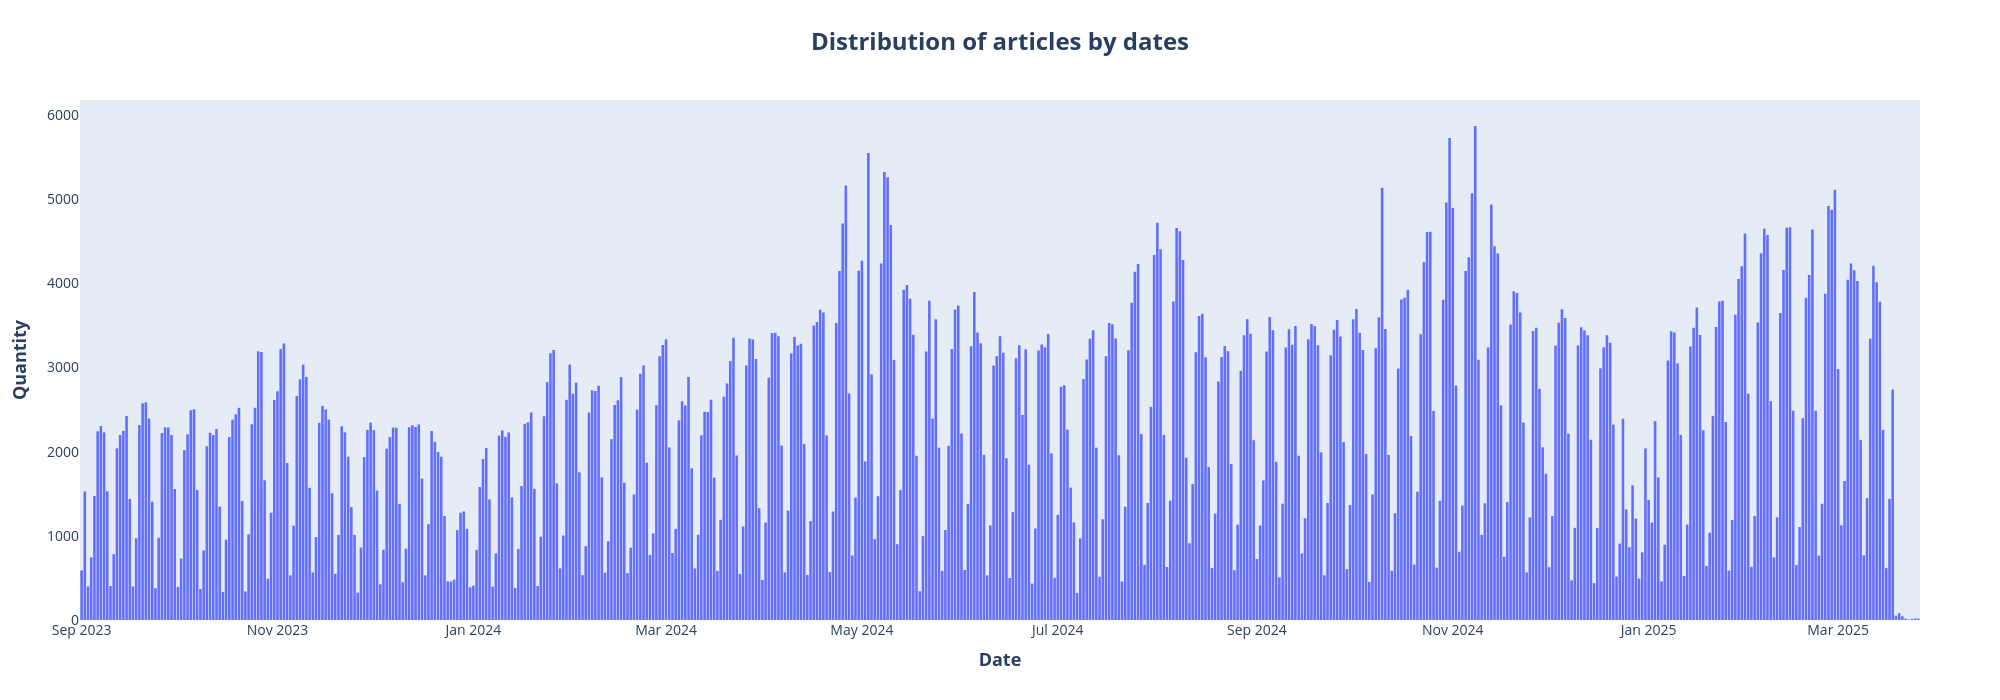
\includegraphics[width=1\linewidth]{img/articles_dist_by_dates.png}
    \caption{Distribution of publications by dates.}
    \label{fig:dist_by_dates}
\end{figure}

\textbf{Distribution of publications by dates.} Figure \ref{fig:dist_by_dates} shows that the number of publications
fluctuates daily with a certain periodicity. A detailed examination revealed that the minimums occur on Sundays and
public holidays, when fewer financial news items are published. This naturally reflects the market’s characteristics:
on weekends and holidays, business activity declines, leading to fewer publications.

\begin{figure}[H]
    \centering
    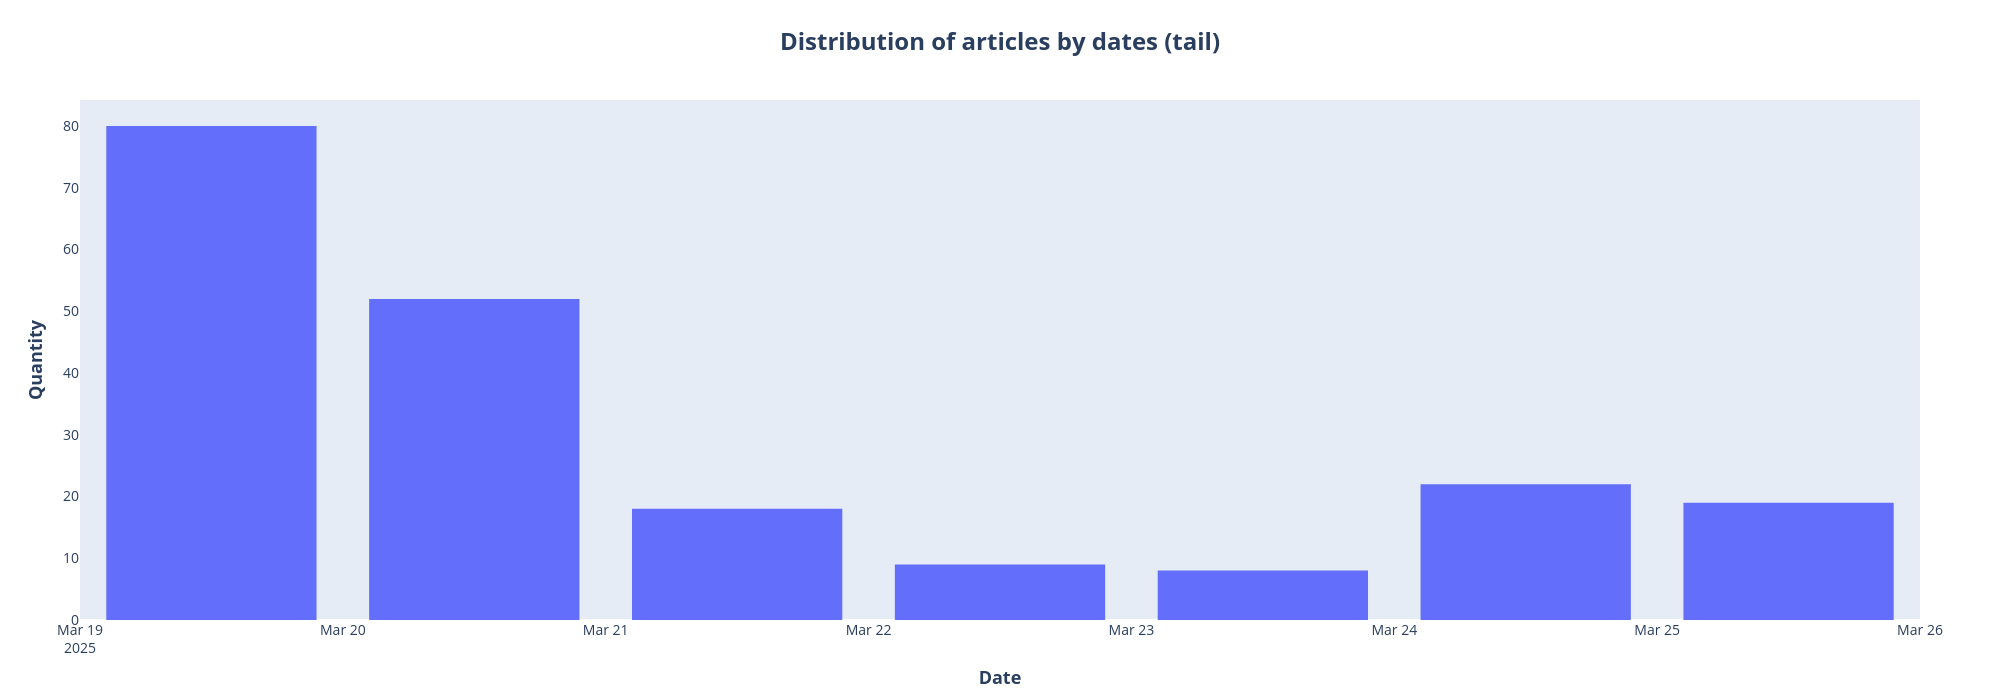
\includegraphics[width=1\linewidth]{img/articles_dist_by_dates_tail.png}
    \caption{\label{fig:dist_by_dates_tail}Distribution of publications by dates (tail).}
\end{figure}

At the same time, some articles, by formal characteristics, fall outside the collection period (September 17, 2023 - March 18, 2025).
Figure \ref{fig:dist_by_dates_tail} displays these "tail" publications, whose count slightly exceeds 200. A more detailed analysis
determined that these articles were indeed published within the specified interval, but their content was later edited or supplemented.
As a result, the publication date and time on the corresponding website were updated, and the old version (with the original date) was
lost. Had the links been parsed not after one week but several weeks later, more such cases would have been observed.

From the perspective of short-term market forecasting, this circumstance may lead to distorted timestamps, making some articles appear
to have been published later than they actually were. Therefore, the dataset might prove less effective for short-term studies compared
to medium- and long-term ones (where a shift of a couple of days is less critical). Nevertheless, for this work it does not play
a crucial role, as the model relies solely on the text of the article and does not take into account the precise publication timestamps.

\begin{figure}[H]
    \centering
    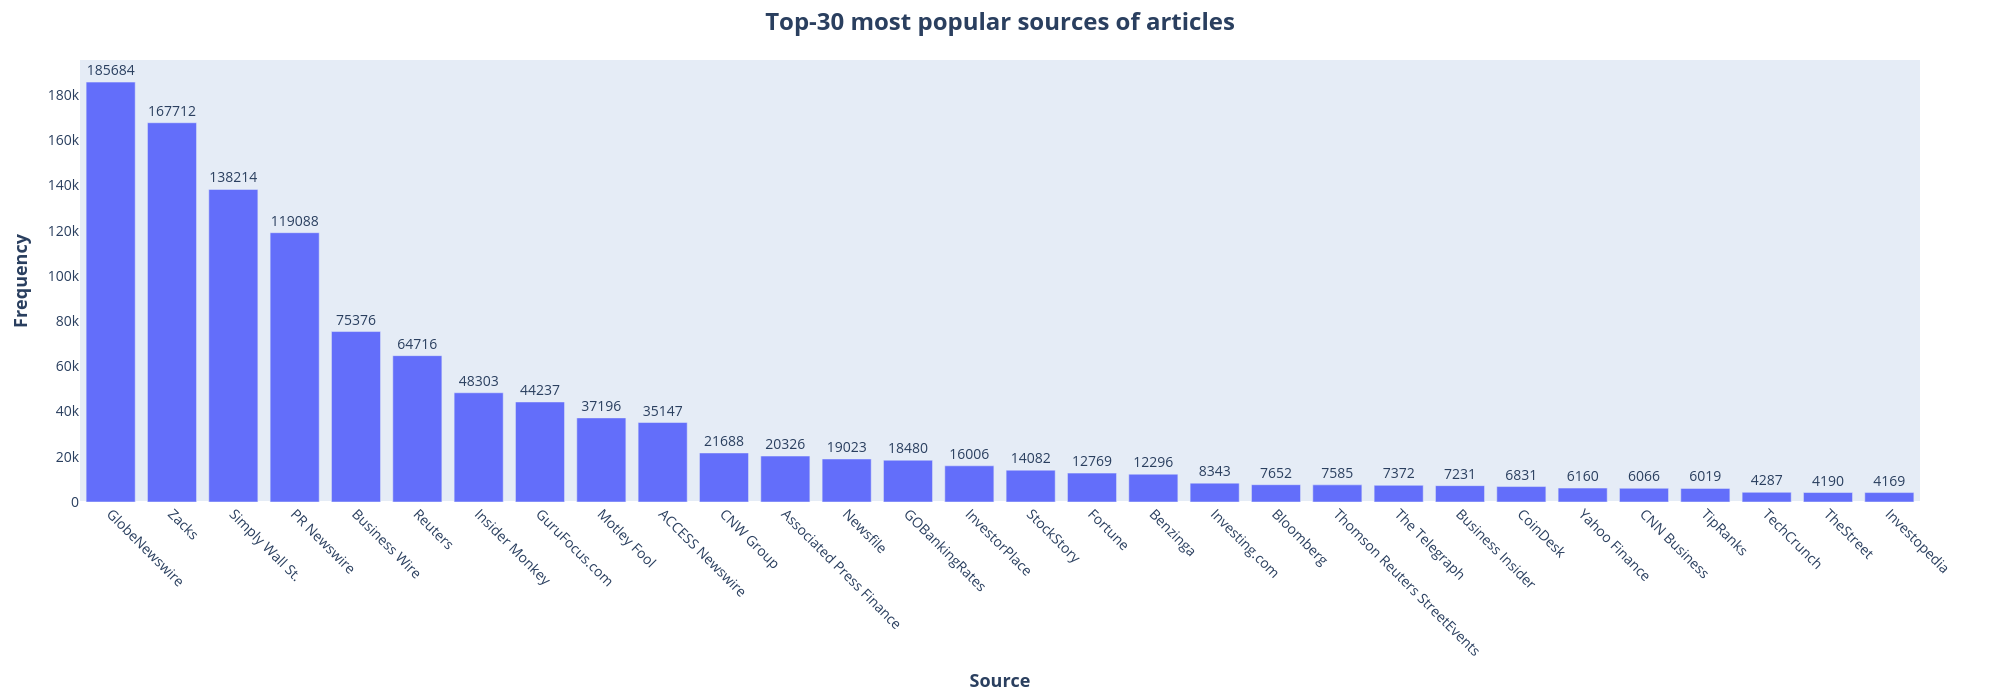
\includegraphics[width=1\linewidth]{img/top30_sources.png}
    \caption{\label{fig:dist_sources}Top-30 most popular sources of publications.}
\end{figure}

\textbf{News Sources.} Figure \ref{fig:dist_sources} illustrates the distribution of publications across the 30 most frequent sources.
The analysis showed that the predominant share of articles (potentially 69.2\%) was published by semi-automated aggregators:
GlobeNewswire, Zacks, Simply Wall St., PR Newswire, Business Wire, GuruFocus.com, Motley Fool, among others. These aggregators focus
on the automatic collection of key data from various resources (regulators, official company websites, etc.), publishing press releases,
brief report summaries, and invitations to corporate events.

Among the top 15 sources, only some can be conditionally considered as "traditional" news outlets, such as Reuters, Insider Monkey,
CNW Group, Associated Press Finance, and InvestorPlace. Meanwhile, outside the top 30, classic publications that primarily publish
original articles prevail. In reality, the blurred boundary between original and semi-automatically generated content complicates
efforts to clearly differentiate them.

According to approximate estimates, out of 1\,300\,000 articles, about 900\,000 (69.2\%) are semi-automated. This is an important factor
for training a language model because:

\begin{enumerate}
    \item The quality of such materials is often lower: texts contain artifacts, broken formatting, and incorrectly inserted characters.
    \item Their volume is large, which, on one hand, provides a substantial sampling capacity, but on the other, complicates cleaning and normalization without the loss of significant information.
\end{enumerate}

Nevertheless, even "imperfect" texts from aggregators convey useful information about the financial market and companies. However,
it is extremely important to develop appropriate cleaning and pre-processing rules (discussed in detail in \hyperref[sec:data_prep]{Section 2.2.4})
to preserve the semantic integrity of the texts.

Furthermore, and perhaps more importantly, these semi-automated texts contribute roughly the same total number of tokens
as the "original" articles (30.8\%), despite their numerical dominance. Consequently, with proper processing, this group of semi-automated
articles can make a significant contribution to training the language model without diminishing the value of the original texts.

\begin{figure}[H]
    \centering
    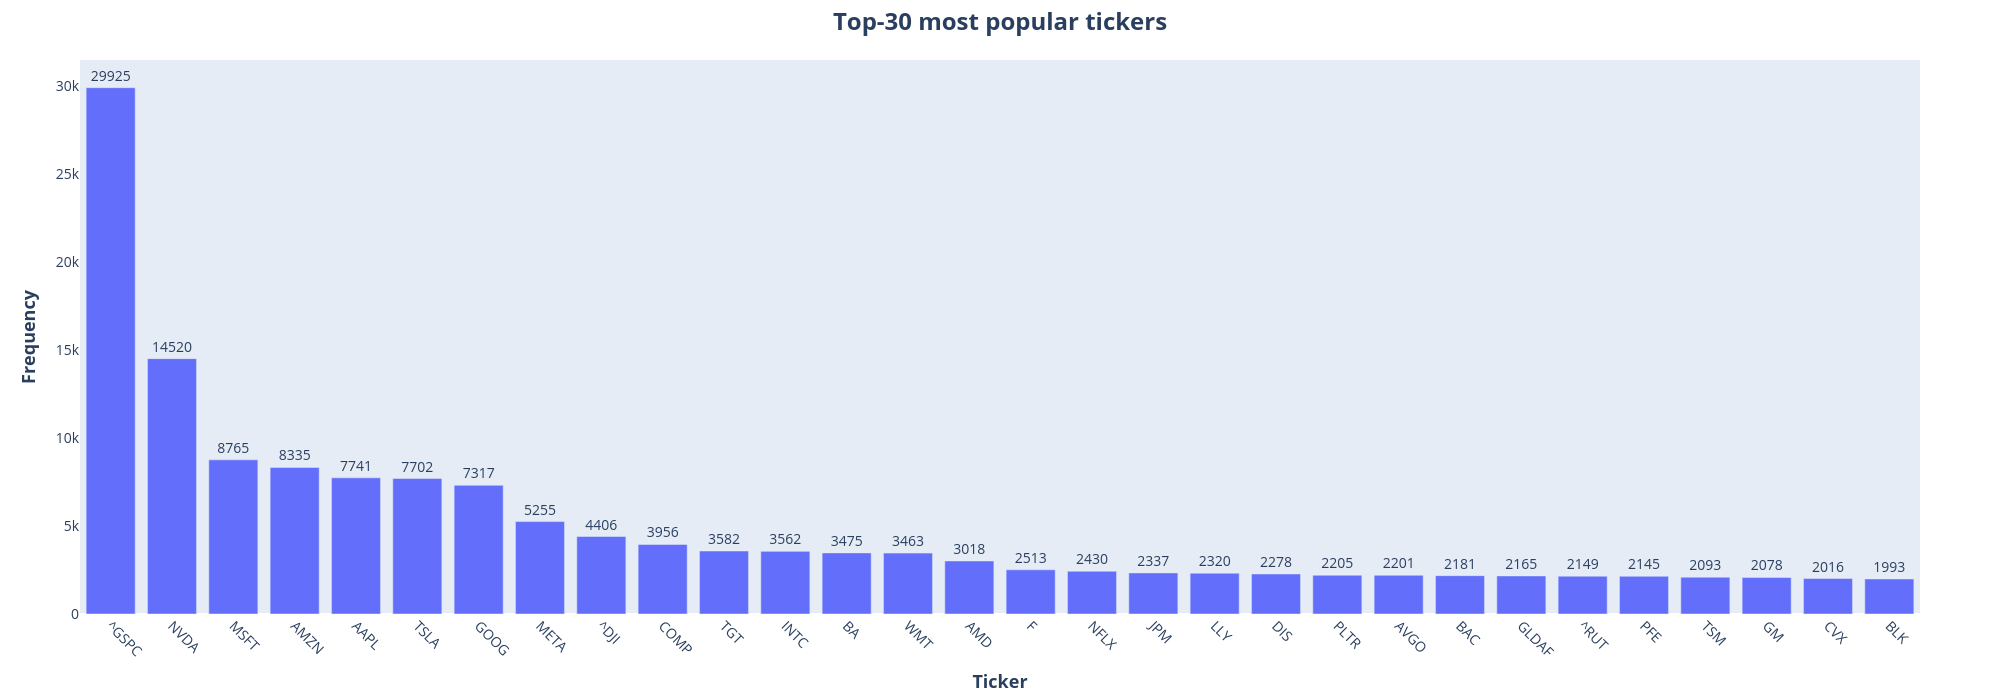
\includegraphics[width=1\linewidth]{img/top30_tickers.png}
    \caption{\label{fig:dist_tickers}Top-30 most popular tickers.}
\end{figure}

\textbf{Analysis of tickers.} Figure \ref{fig:dist_tickers} presents the distribution of publications by the 30 most frequently mentioned
tickers. The leader is the S\&P 500 index, although the sample also includes the Dow Jones and Russell 2000. Notably, the top 10 are predominantly
IT companies, with Nvidia leading by a significant margin.

At the same time, approximately 574\,000 (44.2\%) publications do not contain any tickers in the article header. Moreover, even when tickers
are present, they may not reflect all the companies or indices mentioned in the article. This indicates that although this dataset column
is fairly representative, it does not provide complete coverage of all potential tickers, and some news items are formally omitted
from consideration. Therefore, for tasks beyond the scope of this research, it would be advisable to create a dictionary of terms
and names associated with each specific ticker and then algorithmically augment the ticker column using the corresponding texts.

\begin{figure}[H]
    \centering
    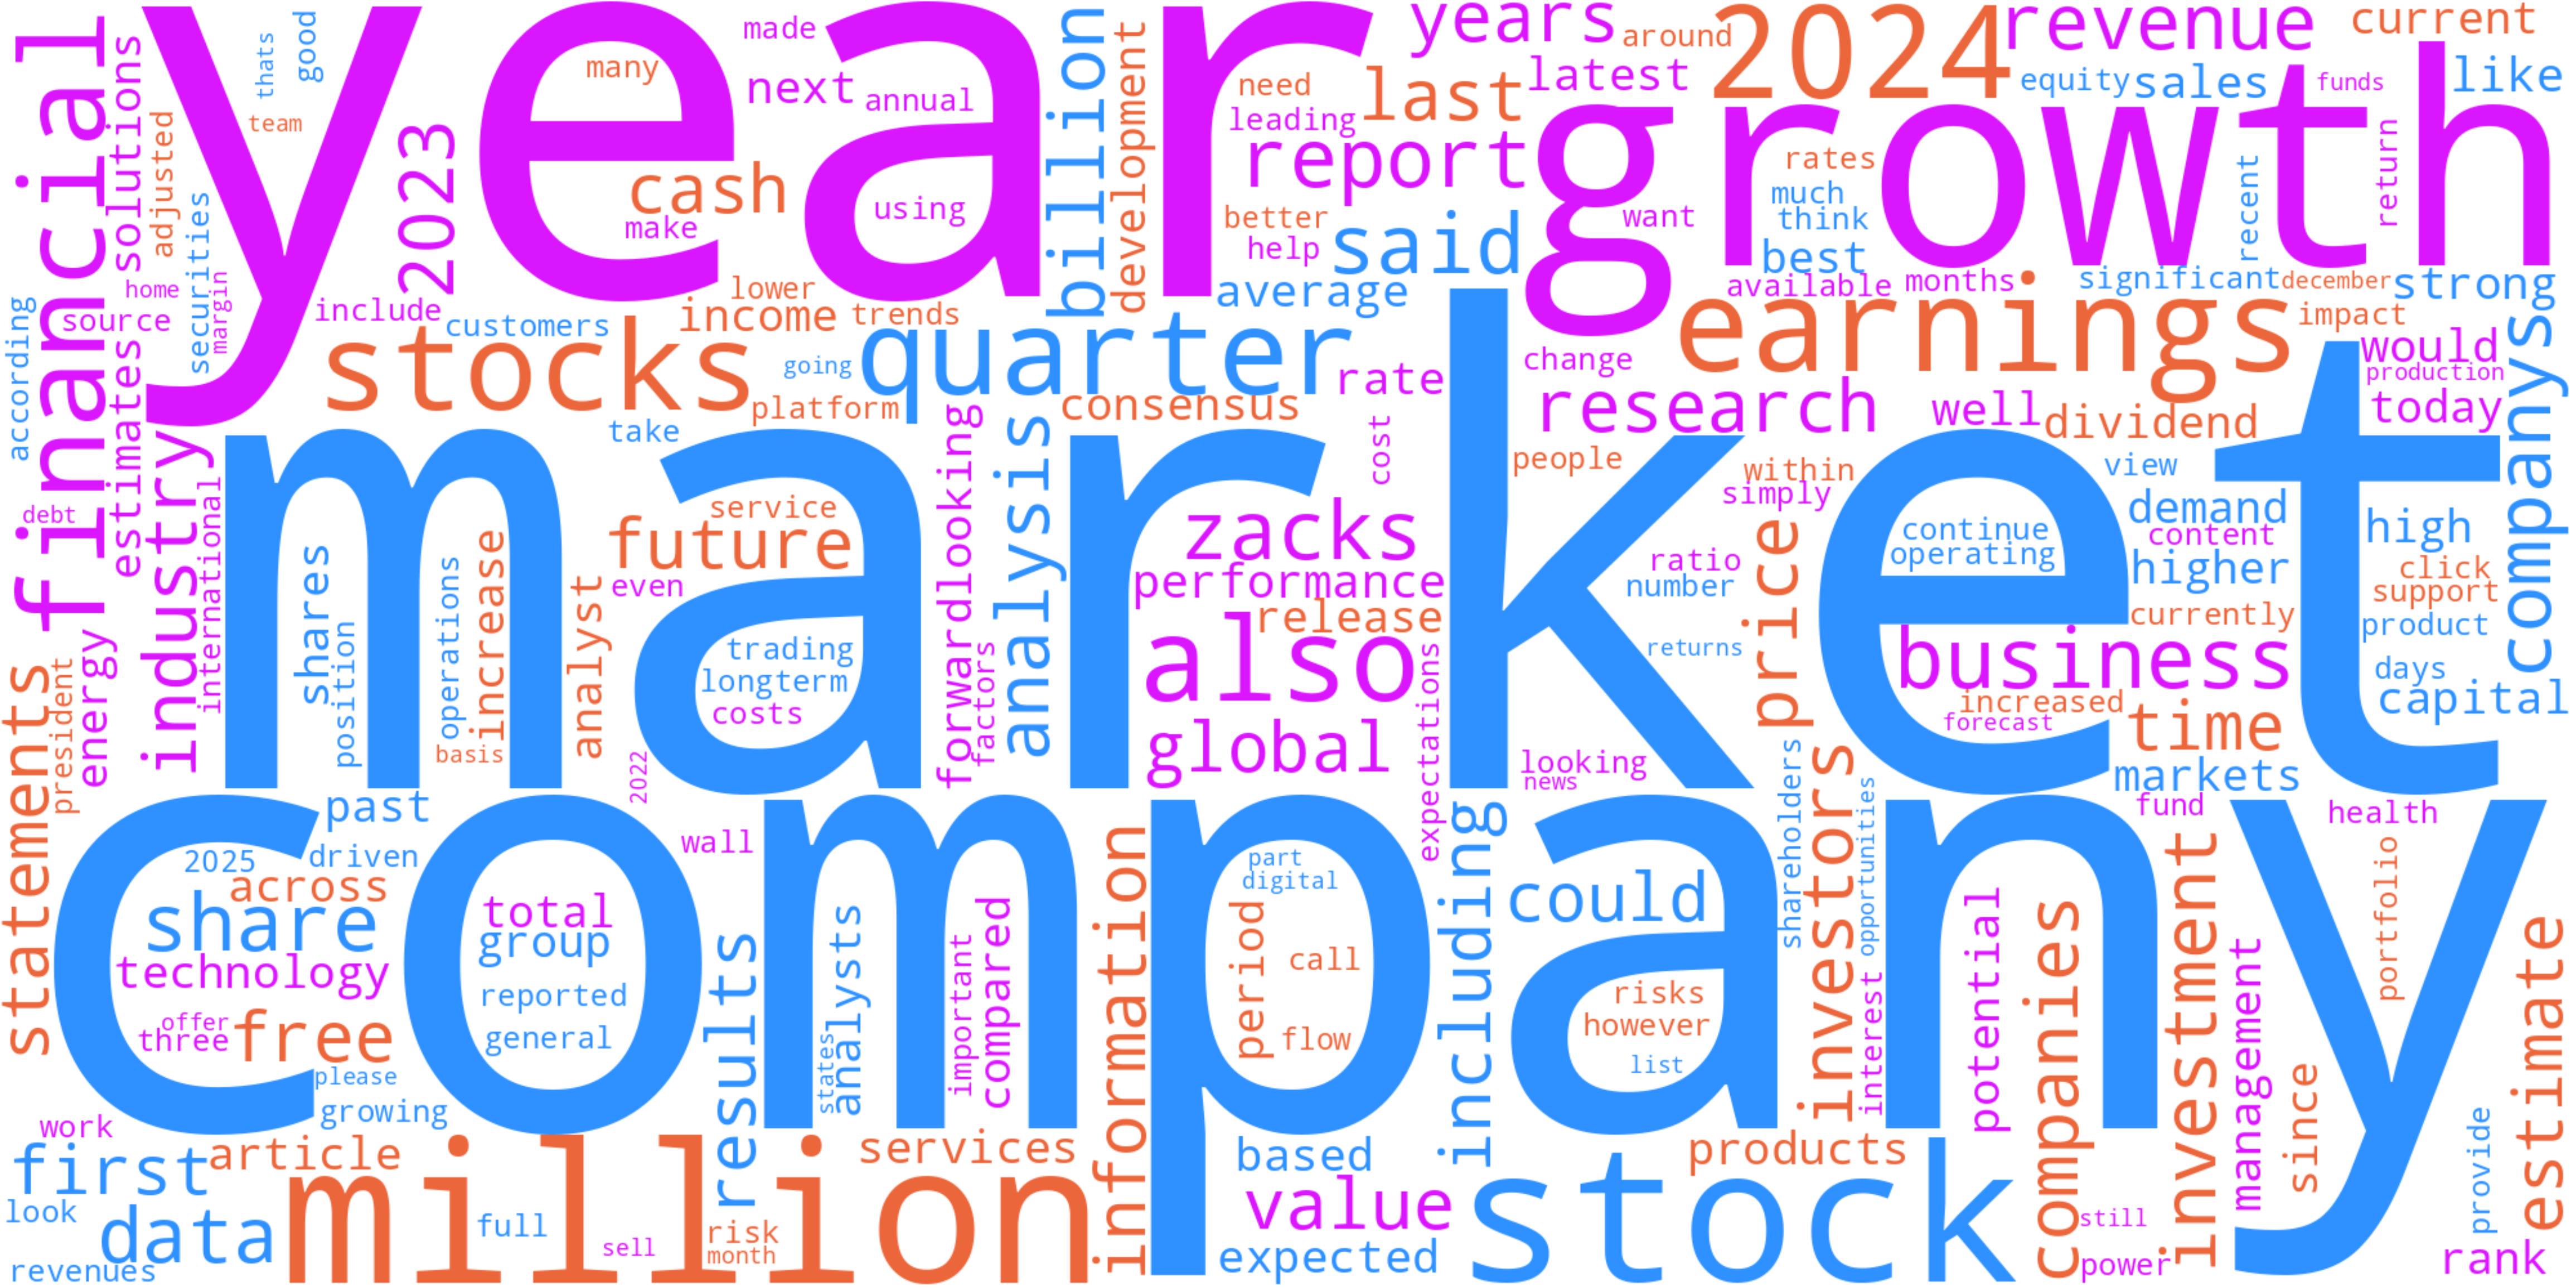
\includegraphics[width=1\linewidth]{img/wordcloud.png}
    \caption{\label{fig:wordcloud}Wordcloud of the whole collected corpus.}
\end{figure}

\textbf{Text Quality.} Figure \ref{fig:wordcloud} shows a word cloud generated from the entire corpus of collected texts.
From this visualization, the following key conclusions can be drawn:

\begin{enumerate}
    \item \textbf{Data Representativeness}. The word cloud demonstrates a wide range of financial terms, indicating that the dataset
    is sufficiently representative of financial topics. This suggests that the material covers various aspects of market activity
    and economic events.
    \item \textbf{Specificity of Financial Terminology}. The frequency distribution of financial terms significantly differs from that observed
    in popular corpora used for training language models (e.g., English Wikipedia or BookCorpus). This discrepancy necessitates the application
    of DAPT to effectively train the model on domain-specific financial data.
    \item \textbf{Level of Noise and Presence of Irrelevant Information}. The word cloud includes elements such as “Zacks”, “click”, “please”,
    “free”, and “source”. This indicates a significant presence of noisy, promotional, or automatically generated fragments, which calls
    for the development of specialized methods for data cleaning without compromising the semantic integrity of the texts.
\end{enumerate}

Additionally, it can be noted that the identified noise and dispersion of terms may negatively affect the quality of downstream tasks,
such as classification or embedding extraction, if the data is not properly processed during the pre-processing stage.

\textbf{Summary}. The collected news dataset is characterized by several notable features. Firstly, there is pronounced seasonality
in the publications—the minimums occur on weekends and public holidays, and so-called "tail" articles have also been recorded.
Secondly, the analysis of sources indicates that about 69\% of the texts originate from semi-automated aggregators, which can complicate
the data cleaning process, as such sources often yield texts with broken formatting, embedded artifacts, and irrelevant information.
Finally, it has been determined that the dataset exhibits a high variability of financial terminology while also containing a significant
level of noise, which altogether confirms the need for DAPT and the development of effective text cleaning
methods.

On one hand, the identified features (time shifts, noise, dominance of semi-automated sources) may reduce the suitability of the dataset
for short-term forecasting or tasks that require precise timestamping. On the other hand, for tasks oriented toward the semantic content
of the text, these issues do not have a critical impact. Proper pre-processing, including text cleaning and the removal of irrelevant
elements, will substantially improve the quality of the trained model and expand its ability to generalize across various types of publications.

\subsubsection{Data Preprocessing}
\label{sec:data_prep}
<<...>>
